\chapter{Understanding source code}

Aesthetics in source code are thus primarily related to cognitive load. In the previous chapter, we've highlighted a focus on understanding when it comes to aesthetic standards: whether obfuscating or illuminating, the process of acquiring a mental model of a given object is a key determinant in the value judgment as applied to source code. In this chapter, we focus on the reason for which such a cognitive load exists in the first place, before surveying the means—both linguistic and mechanistic—that programmers deploy in order to relieve such a load.

This is related to one of the essential features of software: it must be \emph{functional}. As mentioned in our discussion of the differences between source code and software in the introduction, source code is the latent description of what the software will ultimately \emph{do}. Similarly to sheet music, or to cooking recipes\footnote{Recipes are a recurring example taken to communicate the concept of an algorithm to non-experts \citep{zeller_algorithms_2020}}, they require to be put into action in order for their users (musicians and cooks, respectively) to assess their value. Therefore, buggy or dysfunctional software is going to be of less value than correct software \citep{hill_what_2016}, regardless of how aesthetically pleasing the source is.

The assessment of whether a piece of software functions correctly is essentially an assessment of whether what the software does is what the software is supposed to do, which in turn entails knowing what it does, what it is supposed to do, and being able to tell whether these two things are aligned. Any value judgment regarding the aesthetics of the source code at hand would be subject to whether or not the software functions correctly, and such judgment is rendered moot if that software does not work.

After deciding on a benchmark to assess the functionality of the source code at hand (understanding what it should be doing), one must then determine the actual behavior of the source code at hand once it is executed (understanding what it is actually doing). This chapter examines what goes into understanding source code. The first part will lay out our definition of understanding, presenting it as a dual phenomenon, between formalism and contextualism. Starting with 20\^{th} century epistemology, we will see that a dominantly rational, cognitivist perspective on the nature of understanding, as it has been hailed by theoretical computer science research, shows its limits when confronted with practice. Having highlighted this tension, we then turn to how understanding the phenomenon of computation specifically, both on an ontological level, and on a psychological level. The ontological approach will show some of the features of software give it the status on an "abstract artifact", making it a complex object to grasp; the psychological approach will show how such a comprehension takes place for a varity of programmers. Finally, we will conclude with the means that programmers deploy to grasp the concepts at play with software: starting from metaphors used by the general public, we will go down this ladder of abstraction in order to reach the technical apparatuses used in the development and inspection of source code.

The main questions that this chapter addresses are the following: given a certain nature of knowledge acquisition, what are some of the features of computers that make them hard to grasp, and what kind of techniques are deployed in order to address these hurdles and in order to understand what the code is actually doing. This will have us investigate the relationship of knowing and doing, the nature of computation (what is software?) and its relationship to the world as it appears to us (how does modelling and abstraction translate a problem domain into software?), and the cognitive scaffoldings set up to facilitate that task.

% first the definition of understanding
\section{Formal and contextual understandings} %22k char

This section focuses on our definition of understanding—the process of acquiring a working knowledge of an object. Such definition relies on two main aspects: a formal, abstract understanding, and a more subjective, empirical one. We will see how the former had some traction in computer sciences circles, while the second gained traction in programming circles. To support those two approaches, we first trace back the genealogy of understanding in theoretical computer science, before outlining how concrete experience and situatedness outline an alternative tradition.

\subsection{Between formal and informal} %10k

\subsubsection{Theoretical foundations of formal understanding}

To start this inquiry, we go back to the early 20\^{th} century in Cambridge, when the theoretical roots of modern computation were being laid by both philosophers of logic and mathematicians, such as Bertand Russell, Ludwig Wittgenstein, and Alan Turing, as they worked on the formalization of thinking.

Wittgenstein, in particular, bases his argumentation in his \emph{Tractatus Logico-philosophicus} on the fact that much of the problems in philosophy are rather problems of understanding between philosophers—if one were to express oneself clearly, and to articulate one's through clear, unambiguous language, a common conclusion could be reached without much effort:

\begin{quote}
    Most questions and propositions of the philosophers result from the fact that we do not understand the logic of our language. \citep{wittgenstein_tractatus_2010}
\end{quote}

Language and logic are, as we see here, closely connected. Articulated in separate points and sub-points, his work conjugates aphorisms with logical propositions depending on one another, developing from broader statements into more specific precisions. Wittgenstein hints at the intertwining of language as a form of logic, and as logic as a form of language. In this, he follows in the footsteps of Gottfried Leibniz's \emph{Ars Combinatoria}, insofar Leibniz views reasoning and inter-subjective understanding as a formal problem. A universal, and universally-understandable language, called a \emph{characteristica universalis} could resolve any misunderstanding issues. Quoted by Russell, Leibniz notes that:

\begin{quote}
    If we had it [a characteristica universalis], we should be able to reason in metaphysics and morals in much the same way as in geometry and analysis... If controversies were to arise, there would be no more need of disputation between two philosophers than between two accountants [...] Let us calculate. \citep{russell_logical_1950}
\end{quote}

Centuries after Leibniz's declaration, Wittgenstein presents a coherent, articulated theory of meaning through the use of mathematical philosophy, and logic, and his work fits with that of Russell\footnote{In his \emph{Principia Mathematica}, he lays out a theory of logical expression} and Frege\footnote{The \emph{Begriffschrift} similarly attempts to constitute a language in which all scientific statements could be evaluated \citep{korte_frege_2010}, while \emph{Über Sinn und Bedeutung} clarifies the semantic uncertainties between a specific sentence and how it means, or refers to a concept}; even though these are different theories, they are part of a similar endeavour to find a basis od formal propositions through which one could establish truth-values. Such attempt was a direct influence in the work on mathematician Alan Turing—who studied at Cambridge and followed some of Wittgenstein's lectures—, as he developed his own formal system for solving complex, abstract mathematical problems, manifested as a symbolic machine \citep{turing_computable_1936}.

The design of the Turing machine is a subsequent step engagement with the question of understanding in the philosophical sense, as well as in the practical sense—a formal proof to the \emph{Entscheidungsproblem} solved mechanically. Indeed, it is a response to the questions of translation (of a problem) and of implementation (of a solution). This formal approach to instructing machines to operate on logic statements then prompted Turing to investigate the question of intelligence and comprehension in \emph{Computing Machinery and Intelligence}. In it, he translates the hazy term of "thinking" machines into that of "conversing" machines, conversation being a practical human activity which involves listening, understanding and answering (i.e. input, process and output) \citep{turing_computing_2009}. This conversational test, which has become a benchmark for machine intelligence, does rely on the need for a machine to \emph{understand} what is being said. Throughout the article, however, Turing does not yet address the need for a purely formal approach of whether or not a problem can be translated, as Leibniz would have it, into atomistic symbols which would be provided as an input to a digital computer. Such a process of translation would rely on a formal approach, similar to that laid out in the \emph{Tractatus Logico-philosophicus}, or on Frege's formal language described in the \emph{Begriffschrift}. Following a cartesian approach, the idea in both authors is to break down a concept, or a proposition, into sub-propositions, in order to recursively\footnote{although it was not called as such at the time} establish the truth of each of these sub-propositions, and then re-assembled to deduce the truth-value of the original proposition. While Turing focuses on the philosophical and moral arguments to the possibility for machines to think, he does address the issue of artificial intelligence.

With these sophisticated syntactic systems developed a certain approach to cognition, as Turing clearly establishes parallels between the digital computer and the human brain. We now turn to the form of these systems, looking at how their form addresses the problem of clearly understanding and operating on mathematical and logical statements.

Logical calculus, as the integration of the symbol into relationships of many symbols formally takes place through two stylistic mechanisms, the \emph{symbol} and the \emph{list}. Each of the works by Frege, Russell and Wittgenstein quoted above are structured in terms of lists and sub-lists, representing the stylistic pendant to the epistemological approach of related, atomistic propositions and sub-propositions. A list, far from being an innate way of organizing information in humans, is a particular approach to language: extracting elements from their original, situated existence, and reconnecting ways in very rigorous, strictly-defined ways. As Jack Goody writes in \emph{The Domestication of the Savage Mind},

\begin{quote}
    [List-making] [...] is an example of the kind of decontextualization that writing promotes, and one that gives the mind a special kind of lever on 'reality'.\cite{goody_domestication_1977}
\end{quote}

As inventories, early textbooks, administrative documents as public mnemotechnique, the list is a way of taking symbols, pictorial language elements in order to re-assemble them to reconstitute the world, then re-assemble it from blocks, following an assumption that the world can always be decomposed into smaller, discreete and \emph{conceptually coherent} units (i.e. symbols). The list, Goody continues, establishes clear-cut boundaries, they are simple, they are abstract and discontinuous.

Being based on some singular, symbolical entity, applying logical calculus to lists and their symbols, and doing so in a computing environment, becomes the next step in exploring these tools for thinking. Indeed, the engineering development of digital computers in post-war United States as described in \ref{subsec:software-developers}, allowed for the putting into practice of these languages, in the budding field of artificial intelligence (AI).

\subsubsection{Practical attempts at implementing formal understanding}

This putting into practice took the form of subsequent programming languages, relying on a certain conception of human cognition—abstract, logical, as shown above.

IPL, the Information Processing Language, was created by Allen Newell, Cliff Shaw and Herbert A. Simon.  The idea was to make programs understand and solve problems, through "the simulation of cognitive processes" \citep{newell_information_1964}. IPL achieves this with the symbol as its fundamental construct, which at the time was still largely mapped to physical addresses and cells in the computer's memory, and not yet decoupled from hardware.

% add example of IPL
A link between the ideas exposed in the writing of the mathematical logicians and the actual design and construction of electrical machines activating these ideas, IPL was originally designed to demonstrate the theorems of Russell's \emph{Principia Mathematica}, along with a couple of early AI programs, such as the \emph{Logic Theorist}, the \emph{General Problem Solver}. More a proof of concept than a versatile language, IPL was then quickly replaced by LISP as the linguistic means to express intelligence in digital computers.

% add figure on what lisp looks like
LISP (\emph{LIst Processor}) was developed in 1956 was Joseph McCarthy\footnote{McCarthy coined the phrase \emph{Artificial Intelligence} during the 1956 Dartmouth workshop}. The base structural elements of LISP are not symbols, but lists (of symbols, of lists, of nothing), and they themselves act as symbols (e.g. the empty list) \citep{mccarthy_history_1978}. By manipulating those lists recursively—that it, processing something in terms of itself—Lisp shows a tendency for a formal system to separate itself from the problem domain. This is facilitated by its atomistic and relational structure: in order to solve what it has do, it evaluates each symbol and traverses a tree-structure in order to find a terminal symbol, without the explicit need to refer to an external table, for instance.

% add figure on tree structure of language
This sort of heuristic is quite similar to the approach suggested by Noam Chomsky in his \emph{Syntactic Structures}, where he posits the tree structure of language, as a decomposition of sentences until the smallest conceptually coherent parts (e.g. Phrase -> Noun-Phrase + Verb-Phrase -> Article + Substantive + Verb-Phrase). The style is similar, insofar as it proposes a general ruleset (or the at least the existence of one) in order to construct complex structures through simple parts.

Through its direct manipulation of conceptual units upon which logic operations can be executed, LISP became the language of AI, an intelligence conceived first and foremost as logical understanding. The use of LISP as a research tool culminated in the \emph{SHRDLU} program, a natural language understanding program built in 1968-1970 by Terry Winograd which aimed at tackling the issue of situatedness—AI can understand things abtractly through logical mathematics, but can it apply these rules within a given context? The program had the particularity of functioning with a "blocks world" a highly simplified version of a physical environment—bringing the primary qualities of abstraction into solid grasp. The computer system was expected to take into account the rest of the world and interact in natural language with a human, about this world (\emph{Where is the red cube?} \emph{Pick up the blue ball}, etc.). While incredibly impressive at the time, \emph{SHDRLU}'s success was nonetheless relative. It could only succeed at giving barely acceptable results within highly symbolic environments, devoid of any noise. In 2004, Terry Winograd writes:

\begin{quote}
    There are fundamental gulfs between the way that SHRDLU and its kin operate, and whatever it is that goes on in our brains. I don’t think that current research has made much progress in crossing that gulf, and the relevant science may take decades or more to get to the point where the initial ambitions become realistic. \cite{nilsson_quest_2009}
\end{quote}

This attempt, since the beginning of the century, to enable thinking, clarify understanding and implement it in machines, had first hit an obstacle. The world, also known as the problem domain, exhibits a certain complexity which did not seem to be easily translated into singular, atomistic symbols. Around the same time, however, was developed another approach to formalizing the intricacies of cognition.

Warren McCullough's seminal paper, \emph{A logical calculus of the ideas immanent in nervous activity}, co-written with Walter Pitts, offers an alternative based on the embodiment of cognition. They present a connection between the systematic, input-output procedures dear to cybernetics with the predicate logic writing style of Russell and others \citep{mcculloch_logical_1990}. This attachment to input and output, to their existence in complex, inter-related ways, rather than self-contained propositions is, interestingly, rooted in his activy as a literary critic\footnote{Even at the Chicago Literary book club, he argues for a more sensuous approach to cognition: \emph{"In the world of physics, if we are to have any knowledge of that world, there must be nervous impulses in our heads which happen only if the worlds excites our eyes, ears, nose or skin."} \citep{mcculloch_delusion_1953}}.

Going further in the processes of the brain, he indeed finds out, in another paper with Letvinn and Pitts \citep{lettvin_what_1959}, that the organs through which the world excites the brain \emph{are themselves} agents of process, activating a series of probabilistic techniques, such as noise reduction and softmax, to provide a signal to the brain which isn't the untouched, unary, \emph{symbolical} version of the signal input by the external stimuli, and nor does it seem to turn it into such.

We see here the development of a theory for a situated, embodied stance towards cognition, which would ultimately resurface through the rise of machine learning via convoluted neural networks in the 2000s \citep{nilsson_quest_2009}. In it, the senses are as essential as the brain for an understanding—that is, for the acquisition, through translation, of a conceptual model which then enable deliberate and successful action. It seems, then, that there are other ways to know things than to rely on description through formal propositions.

\vspace*{1\baselineskip}

A couple of decades later, Abelson and Sussman still note, in their introductory textbook to computer science, the difficulty to convey meaning mechanically:

\begin{quote}
    Understanding internal definitions well enough to be sure a program means what we intend it to mean requires a more elaborate model of the evaluation process than we have presented in this chapter. \citep{abelson_structure_1979}
\end{quote}

While formal notation is able to enable digital computation, it nonetheless proved to be limited when it came to accurately and expressively  conveying meaning. This limitation, of being able to express formally what we understand intuitively (e.g. \emph{what is a chair?}\footnote{A question addressed by Joseph Kosuth in his artwork \emph{One and Three Chairs}, 1965}) appeared as computers applications left the domain of logic and arithmetic, and were applied to more social domains.

After having seen the possibilities and limitations of making machines understand through the use of formal languages, and the shift offered by taking into account sensory perception as a possible locus of cognitive processes, we now turn to these ways of knowing that exist in humans in a more embodied capacity.

% todo
% \begin{itemize}
    % \item EXAMPLE: XML (applen, mcdaniel, rhetorics of xml)
% \end{itemize}

\subsection{Knowing-what and knowing-how} %10k

1953 saw a radical posture change from one of the logicians whose work underpinned AI research, briefly before the start of these attempts to implement artificial intelligence in digital computers. This was the publication of Wittgenstein's \emph{Philosophical Investigations}. In his second work, he disown his previous approach to language as seen in the \emph{Tractatus Logico-philosophicus}, and favors a more contextual, use-centered frame. Rather than what knowledge is, he looks at how knowledge is acquired and used; while (formal) lanuage was previously defined as the exclusive means to translation concepts in clearly understandable terms, he broadens his perspective in the \emph{Inquiries} by stating that language is \emph{"the totality of language and the activities with which it is intertwined"} and that \emph{"the meaning of a word is its use within language"} \citep{wittgenstein_recherches_2004}, noting context and situatedness as a important factors in the understanding process.

At first, then, it seemed possible to make machines understand through the use of formal languages. The end of the first wave of AI development, as a branch of computation specifically focused on cognition, have shown some limits to this approach.  We now turn to theories which support this approach of an embodied and contextualized knowing, complemented by a constructivist approach to building an understanding.

% 4000
\subsubsection{Knoweldge and situation}

As hinted at by the studies of McCullough and Levitt, understanding a situation doesn't rely exclusively on abstract logical processes, but also on the processes involved in grasping this situation, such as, in their case, peripheral vision processing. It is not just what things are, but how they are, and how they are \emph{perceived}, which matters. Different means of inscription and description do tend to have an impact on the ideas communicated and understood.

In his book \emph{Making Sense: Cognition, Computing, Art and Embodiment}, Simon Penny refutes the so-called unversality of formulating cognition as a formal problem, and develops an alternative history of cognition, akin to Michel Foucault's archeology of knowledge. Drawing on the works of authors such as William James, Jakob von Uexküll and Gilbert Ryle, he refutes the Cartesian dualism thesis which acts as the foundation of AI research \citep{penny_making_2019}. A particular example of the fallacy of dualism, is the use of the phrase \emph{implementation details}, which he recurringly finds in the AI literature, such as Herbert Simon's \emph{The Sciences of the Artificial} \citep{simon_sciences_1996}. The phrase refers to the gap existing between the statement of an idea, of an algorithm, and a procedure, and its concrete, effective and functional manifestation.

For instance, pseudo-code is a way to sketch out an algorithmic procedure, which might be considered agnostic when it comes to implementation details. One can consider the pseudo-code in \ref{code:nielsen_chalktalk}, which describes a procedure to recognize a free-hand drawing and transform it into a known, formalized glyph. Disregarding the implementation details means disregarding any reality of an actual system: the operating system (e.g. UNIX or MSDOS), the input mechanism (e.g. mouse, joystick, touch or stylus), the rendering procedure (e.g. raster or vector), or the programming language (e.g. JavaScript or Python).

\begin{listing}
    \begin{minted}{python}
        recognition = false
        do until recognition
        wait until mousedown
            if no bounding box, initialize bounding box
            do until mouseup
            update image
            update bounding box
            rescale the material that's been added inside
            if we recognize the material:
                delete image from canvas
                add the appropriate iconic representation
                recognition = true
    \end{minted}
    \caption[]{Example of pseudo-code attempting to reverse-engineer a software system, ignoring any of the actual implementation details, taken from \citep{nielsen_working_2017}}
    \label{code:nielsen_chalktalk}
\end{listing}

Refuting the idea that pseudo-code is all that is necessary to communicate and act upon a concept, Penny  argues on the contrary that information is relativistic and relational; relative to other pieces of information (intra-relation) and related to contents and forms of presenting this relation (extra-relation). Pseudo-code will only ever make sense in a particular implementation context, which then affects the product.

He then follows Philip Agre's statement that a theory of cognition based on formal reason works only with objects of cognition whose attributes and relationships can be completely characterized in formal terms; and yet a formalist approach to cognition does not prove that such objects exist or, if they exist, that they can be useful. Uses of formal systems in artificial intelligence in specific, and in cognitive matters in general, is yet another instance of the map and the territory problem—it only goes so far.

Beyond the syntax of formal logic, there are different ways to transmit cognition in actionable form, depending on the form, the audience and the purpose. In terms of form, a symbol system of formal logic is only one of many possibilities for systems of forms. In his \emph{Languages of Art}, Nelson Goodman elaborates a theory of symbol systems, which he defines as formal languages composed of syntactic and semantic rules \citep{goodman_languages_1976}. Logical notation exists along with music, painting, poetry and prose. What follows, argues Goodman, is that all these formal languages involve an act of \emph{reference}. Through different means (exemplification, denotation, resemblance, representation), formal systems act as sets of symbols which can denote or exemplify or refer to in more complex and indirect ways, yet always between a sender and a receiver\footnote{Understood as the eponymous entities  in Jakobsen's model of communication functions.}.

Communication, as the transfer of meaning from one individual to one or more other individuals, does not exclusively rely on the use of mathematical based use of formal languages. From Goodman to Goody, the format of representation also affords differences in what can be thought and imagined. Something that was always implicit in the arts—that representation is a complex and ever-fleeting topic—is shown more recently in Marchand-Zañartu and Lauxerois's work on pictural representations made by philosophers, visual artists and novelists (such as Claude Simon's sketches for the structure of his novel \emph{La Route des Flandres}, shown in \ref{image:routedesflandres}) \citep{marchand-zanartu_32_2022}. How specific domains, from mathematics to visual arts and construction, engage in the relation between form and cognition is further adressed in CHAPTER\_4.

\begin{figure}
    \begin{center}
        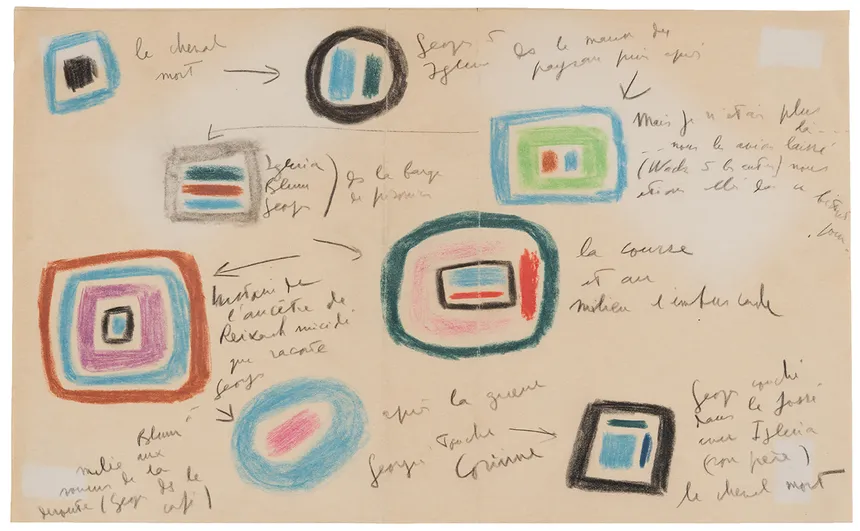
\includegraphics[width=\textwidth,height=\textheight,keepaspectratio]{routedesflandres.png}
        \caption{Tentative d'organisation visuelle pour le roman La Route des Flandres, années 1960 - Claude Simon, écrivain}
        \label{image:routedesflandres}    
    \end{center}    
\end{figure}

Going beyond logical notation, we have seen that there are other conceptions of knowledge which take into account the physical, social and linguistic context of an action. Nonetheless, these can still be systematized, as Goodman highlights in his investagation of referential systems, with a focus on reference of the ideas at hand.

% 4000
\subsubsection{Constructing knowledge}

There are multiple ways to express an idea: on can use formal notation or draft a rough sketch with different colors. These all highlight different degrees of expression, but one particular way can be considered problematic in its ambition. Formal languages rely on the assumption, that all which can be known can ultimately be expressed in unambiguous terms. First shown by Wittgenstein in the two main eras various eras of his work, we know focus on the ways of knowing which cannot be explicited.

First of all, there is a separation between \emph{knowing-how} and \emph{knowing-that}; the latter, propositional knowledge, does not cover the former, practical knowledge, as shown by Ryle \citep{ryle_concept_1951}. Perhaps one of the most obvious example of this duality is in the failure of Leibniz to construct a calculating machine, as told by Matthew L. Jones in his book \emph{Reckoning with Matter}. In it, he traces the history of philosophers to solve the problem of constructing a calculating machine, a problem which would ultimately be solved by Charles Babbage, with the consequences that we know \citep{jones_reckoning_2016}.

Jones depicts Leibniz in his written correspondence with watchmaker Ollivier, in their fruitless attempt to construct Leibniz's design; the implementations details seem to elude the German philosopher as he refers to the "confused" knowledge of the nonetheless highly-skilled Parisian watchmaker. The (theoretical) plans of Leibniz do not match the (concrete) plans of Ollivier.

These are two complementary approaches to the knoweldge of something: to know \emph{what} constructing calculating machine entails and knowing \emph{how} to construct such a machne. In the fact that Ollivier could not communicate clearly to Leibniz what his technical difficulties, we can see an instance of something which would be theorized centuries later by Michael Polanyi as \emph{tacit knowledge}, knowledge which cannot be entirely made explicit.

Polanyi, as a scientist himself, starts from another assumption: we know more than we can tell. In his eponymous work, he argues against a positivist approach to knowledge, in which empirical and factual deductions are sufficient to achieve satisfying epistemological work. What he proposes, derived from \emph{gestalt} psychology, is to consider some knowledge of an object as the knowledge of an integrated set of particulars, of which we already know some features, by virtue of the object existing in an external approach. This integrated set, in turn, displays more properties than the sum of its parts. While formal notation suggests that the combination of formal symbols does not result in additional knowledge, Polanyi rather argues, against Descartes, that relations and perceptions do result in additional knowledge. 

\begin{quote}
    The knowledge of a problem is, therefore, like the knowing of unspecifiables, a knowing of more than you can tell. \citep{polanyi_knowing_1969}
\end{quote}

Rooted in psychology, and therefore in the assumption of the embodimed of the human mind, Polanyi posits that all thought is incarnate, that it lives by the body and by the favour of society, hence giving it a physio-social dimension. This confrontation with the real-world, rather than being a strict hurdle that has to be avoided or overcome, as in the case of SHRDLU above, becomes one of the two poles of cognitive action. Knowledge finds its roots and evaluation in concrete situations, as much as in abstract thinking. In the words of Cecil Wright Mills, writing about his practice as a social scientist research,

\begin{quote}
    Thinking is a continuous struggle between conceptual order and empirical comprehensiveness. \citep{MillsC.WrightCharlesWright2000Tsi}
\end{quote}

Polanyi's presentation of a form of knowledge following the movement of a pendulum, between dismemberment and integration of concepts finds an echo in the sociological work of Mills: a knowledge of some objects in the world happens not exclusively through formal descriptions in logical symbol systems, but involves imagination and phenomenological experience—wondering and seeing. This reliance on vision—starting by recognizing shapes, as Polanyi states—directly implies the notion of aesthetic assessment, such as a judgement of typical or non-typical shapes. He does not, however, immediately elucidate how aesthetics support the formation of mental models at the basis of understanding, only that this morphology is at the basis of higher order of represenations.

Seeing, though, is not passive seeing, simply noticing. It is an active engagement with what is being seen. Mills's quote above also contains this other aspect of Polanyi's investigation of knowledge, and already present in Ollivier's relation with Leibniz: knowing through doing.

This approach has been touched upon from a practical programmer's perspective in section \ref{subsec:craft-knowledge}, through a historical lens but it does also posses theoretical grounding. Specifically, Harry Collins offers a deconstruction of the Polanyi's notion by breaking it down into \emph{relational}, \emph{somatic} and \emph{collective} tacit knowledges \citep{collins_tacit_2010}. While he lays out a strong approach to tacitness of knowledge (i.e. it cannot be communicated at all), his distinction between relational and somatic is useful here\footnote{His definition of collective tacit knowledge touches on the knowledge present in any living species and is impossible to ever be explicited, and is therefore out of scope here.}. It is possible to think about knowledge as a social construct, acquired through social relations: learning the linguo of a particular technical domain, exchanging with peers at conferences, imitating an expert or explaining to a novice. Collective, unspoken agreements and implicit statements of folk wisdom, or implicit demonstrations of expert action are all means of communication through which knowledge gets replicated across subjects.

Concurrently, somatic tacit knowledge tackles the physiological perspective as already pointed out by Polanyi. Rather than knowledge that exists in one's interactions with others, somatic tacit knowledge exists within one's physical perceptions and actions. For instance, one might base one's typing of one's password strictly on one's muscle memory, without thinking about the actual letters being typed, through repetition of the task. Or one might be spotting a cache bug which simply requires a machine reboot, due to experience machine lifecycles, package updates, networking behaviour. Not completely distinct from its relational pendant, somatic knowledge is acquired through experience, repetition and mimeomorphism—replicating actions and behaviours, or the instructions, often under the guidance of someone more experienced.

\vspace*{1\baselineskip}
\centerline{\rule{0.13334\linewidth}{.4pt}}
\vspace*{1\baselineskip}

We started our discussion of understanding by defining it as the acquisition of the knowledge of a object—be it a concept, a situation, an individual or an artfefact,, which is accurate enough that it allows us to predict the behaviour and to interact with such object. Within this defintion, one could take the example of a human discussion as a demonstration of advanced understanding, as something that is both situated, and formalized.

Theories of how individuals acquire understanding (how they come to know things, and know conceptual representations of things), have been approached from an explicit perspective, and an implicit one. In the rationalist, logical philosophical tradition, we have seen that the belief that meaning can be rendered unambiguous through the use of specific notation. This has led to the development of logic and computer science, as this meaning got mechanized. Explicit understanding is therefore the theoretical lineage of computation.

However, as we've seen in the first hurdles of artificial intelligence research, explicit specification of meaning falls short of handling everyday tasks which humans would consider to be menial. This has led us to consider a more implicit approach to understanding, in which it is acquired by tacit means. Particularly, we've identified this tacit knowledge as relying on a social component, as well as on a somatic component.

Source code, as a formal system with a high dependence of context, intent and implementation, mobilizes both approaches to understanding. Before we dive deeper about how these two modes of understanding are mobilized at the end of this chapter, we now turn to what makes computation a cognitively complex object, and what are some cognitive reactions that humans display in situations where they have to understand, and work with, software.

\clearpage

% first the computer
\section{Understanding computation}

\centerline{\rule{1\linewidth}{.4pt}}

the sections below are still in the state of rough notes

\centerline{\rule{1\linewidth}{.4pt}}

We've laid out the groundwork by showing that there are multiple ways to understand something. We now turn to the thing we want to understand. What makes it challenging to understand computation?

First, we will look at it from a more abstract point of view, investigating the ontological status of software. This will highlight some of the theoretical properties that make it hard to understand, such as its relation to hardware, its relation to a specification, and its relation to time and space.

Second, we will look at the practical investigations of how people understand software by looking into the psychology and cognition of programmers, with various studies and books on the subject. This will give us a better picture of the process which aesthetics in source code are supposed to influence.

% the software effect (combination of knowing what (it does) and how (it does it))
% the philosophical enquiries

\subsection{Software ontology} %11k

The first section focuses on technology, with simondon expliciting an ambiguous status. This ambiguous status is then further looked at through the concept of the "abstract artifact". That is, they are syntactic entities which exhbit artefactual properties (that is, it has spatio-temporal properties). Artefact A is an implementation in medium M of the definition F.

It's always conceptually designed and materially implemented. To use Cantell-Smith's phrase, it's \emph{meaning mechanically realized}, at the interaction of two traditions: logical and mechanical.

this 'dynamic of organized inorganic matter' (Stiegler 1998: 84). \url{http://tapoc.sourceforge.net/progress/2012/06/notes_for_berry-philosophy_of_software.html} p.4

Technical artefacts have \emph{functional} properties (purpose) and \emph{structural} ones (physical makeup which allow for the completion of the functional purpose) \citep{turner_computational_2018}

\begin{itemize}
    \item lando, lapujade, towards a general ontology of computer programs
    \item irmak, software is an abstract artifact
    \item suber, what is software
    \item cantell smith age of significance introduction
    \item berry philosophy of software
    \item turner, computational artifacts
    \item rapaport
    \item simondon
    \item kirsch, maglio, distinguish epistemic from pragmatic action
\end{itemize}

\subsubsection{Software complexity}

The dynamic notion of a state of a process \citep{rapaport_philosophy_2005}. It is an epistemic action.

a program is a \emph{cognitive artefact}, which can be understood on three different levels, according to Moor \citep{moor_three_1978}:

\begin{itemize}
    \item the physical level (transistors)
    \item the design level (specifications, effective)
    \item the intent level (the goal and desire)
\end{itemize} 

There are different types of complexity that we can develop further

\begin{itemize}
    \item conceptual complexity \citep{lando_general_2007}
    \item modeling complexity \citep{lando_general_2007}
    \item temporal complexity (issues of speed, sequentiality and parallelism, there is a qualitative change when operations are executed millions of times per second)
    \item spatial complexity (the network)
\end{itemize}

\begin{quote}
    Code is therefore technical and social, and material and symbolic simultaneously. Rather, code needs to be approached in its multiplicity, that is, as a literature, a mechanism, a spatial form (organization), and as a repository of social norms, values, patterns and processes. \citep{berry_philosophy_2011} (pp 36-37)
\end{quote}

The problem, again, is that programming is an information management technique which, in turn, produces information.

In order to understand a computer program, we need to give it meaning, that's what always happens: "distinguishing from noise is something that literature does" (Suber, 1988, p.97). Such that the question "what does a Turing machine do?" has `n+1` answers. 1 syntactic, and n semantic (however many interpretations) \citep{rapaport_philosophy_2005}.

\subsection{The psychology of programming} %11k
% the studies

So software is complicated. How do individuals deal with it? Constructing, and understanding it? The idea is to start how this happens empirically, i.e. looking at programmers' cognitive activities.

\begin{itemize}
    \item \citep{petre_glimpse_1997} is one of the earliest studies found, based on previous anecdotal evidence
    \item \citep{detienne_software_2012} more extensive overview of the research in psychology in programming, introducting concepts such as the modeling of knowledge (further qualifying petre), beacons, and surface-structure vs. deep-structure.
    \item \citep{ivanova_comprehension_2020}, comprehension of computer code, is the most recent, and further complicates the narrative (no pun intended) by showing no clear association with the text-processing part of the brain and the code-processing part of the brain
    \item \citep{weinberg_psychology_1998} is more of a business literature perspective, but is included for good measure, specifically to highlight that a lot of these studies were based on a software developer perspective.
\end{itemize}

Turner states that agency determines what the function is (i can use the computer as a doorstop): it is the difference between specification (intent-free) and semantic interpretation (intent-rich); one can dictate the other (and vice versa!). \citep{turner_computational_2018} This intentional model is an extension of the mental-model approach (aka programmers don't care about theory, they just do and tinker). there are no norms and this is hell for a logician.

% then the human mind
\section{Means of understanding}

As we've seen in the previous sequence, there are specific problems to understanding computation, but there are also ways of achieving a good understanding of a program, specifically metaphors and tools.

We'll spend most of this section looking at the ubiquity of metaphors in computing, as a cognitive mechanism, relying on the work of Lakoff and Johnson, both from users and programmers. We will also investigate the concrete use of extensions of mind through software tools, particularly on the role of \emph{Integrated Development Environments} (IDEs).

% then the communcation between both
\subsection{Metaphors of computation}

Here we include the section in the 4th report about metaphors in computation.

But we will also need more practical examples.

\begin{itemize}
    \item sally wyatt
    \item chun, on the persistence of visual knowledge
    \item a first pass on interfaces as metaphors (nielsen, galloway)
    \item cramer and fuller in \emph{Software studies}
    \item lakoff (ricoeur will come when we talk about PLs)
    \item example about the clipboard
\end{itemize}

\subsection{Tools as an extension}
% IDEs

\begin{itemize}
    \item extended mind hypothesis of clark and chalmers (1998)
    \item fishwick aesthetic progamming
    \item allamanis, using ML for code generation and analysis, and mattt (as we may code) highlights the need for such a thing (quoting: What if, instead of lowering source code down for the purpose of execution, we raised source code for the purpose of understanding?)
    \item barker writing software documentation
    \item wilken card index
\end{itemize}

% The computer as prosthetic organ, distributed cognition

\pagebreak

Conclusion: we circle back to aesthetics, particularly relying on \citep{dexter_embodied_2011} and we look at the things that are both tools and metaphors: programming languages. We will see what roles metaphors play; and, if linguistics is a key component in the writing of clear source code, we should also look at programming languages.